\subsection{Issues}
The project didn't go as smoothly as we had hoped. The group agreed on pretty much everything, but the issues we had were mostly related to the software and tools not cooperating or working as we expected.

\subsubsection{C\# Compiler}
When we tried to add the database to our project via the entity framework we had troubles with the C\# compiler not being found. This was due to the installation of the Visual Studio 2012 Release candidate edition (which had expired), so we had to uninstall this RC version to install the "normal" Visual Studio 2012 which lead to the compiler not working - we couldn't add new items, compile or make a new project
There was however a quickfix to repair the compiler by using the gacutil utility software included with Visual Studio 2012.
This command in cmd fixed it:
\begin{verbatim}
gacutil /u Microsoft.VisualStudio.CSharp.Services.Language.Interop 
\end{verbatim}

\subsubsection{GitHub DDoS}
On October 14, the day of the midterm delivery, GitHub experienced a DDoS attack. This resulted in some of the files we were working on for the report becoming locked mid-commit and mid-pull, and preventing us from performing a new git pull. This also prevented some of us from compiling, due to a previous commit containing errors having been pulled.

\subsubsection{Windows on Mac}
Mac is not Windows. %TODO Truls

\subsubsection{SDM}
NTNU gurutjeneste offers free MSDNAA account which we can use to download Microsoft software from MSDN software center (Microsoft developer network). To download software from MSDN we had to use Secure Download Manager (from now on referred to as SDM), by opening the .SDX file obtained from the MSDN webpage. The download went find however the unpacking of the files gave us an unknown error without further information.
\begin{figure}[H]
\centering
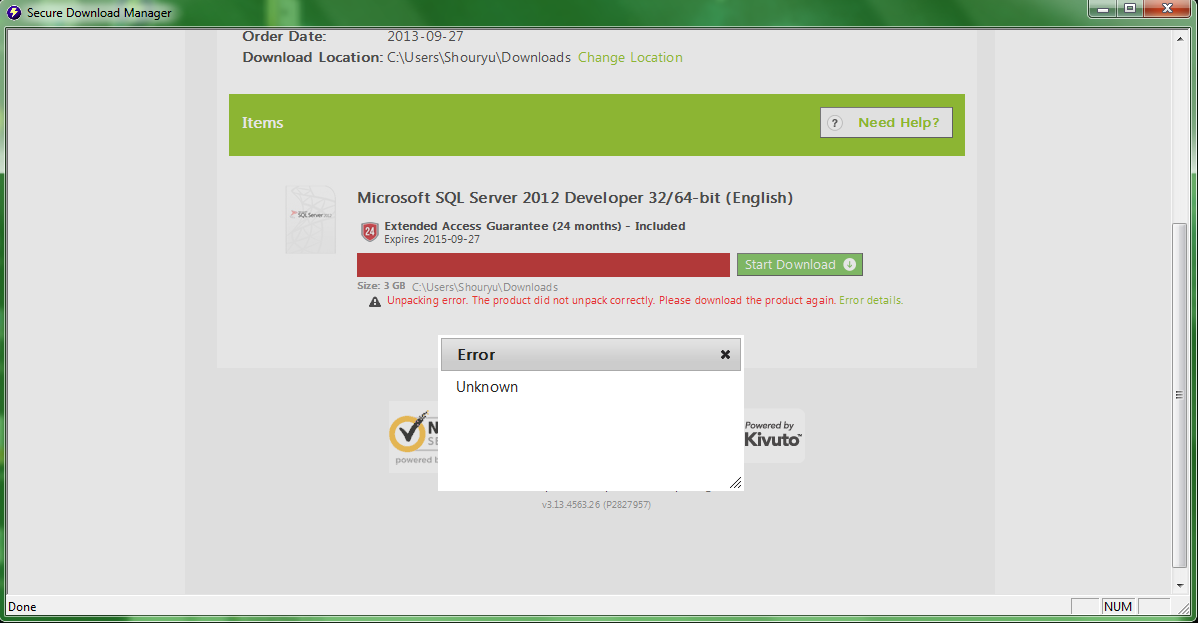
\includegraphics[width=0.8\textwidth]{images/issue00.png}
\caption{SDM error}
\label{fig:SDM_error}
\end{figure}

\subsubsection{MSSQL}
DB


